\subsubsection{usergoal-ugManageCrisis}

\label{RE-use-case-ugManageCrisis}



The goal is to do an action that makes the handling of a crisis or an alert progress. 


\begin{usecase}
  \addheading{Use-Case Description}
  \addsingletwocolumnrow{Name}{ugManageCrisis}
  \addsingletwocolumnrow{Scope}{system}
  \addsingletwocolumnrow{Level}{usergoal}
  

\addrowheading{Primary actor(s)}
\addnumberedsinglerow{}{\msrcode{actCoordinator[active]}}
\addnumberedsinglerow{}{\msrcode{actActivator[proactive]}}



\addrowheading{Goal(s) description}
\addsinglerow{
The goal is to do an action that makes the handling of a crisis or an alert progress. 
}

\addrowheading{Reuse}
\addnumberedsinglerow{}{\msrucname{oeValidateAlert [0..*]}}
\addnumberedsinglerow{}{\msrucname{oeSetCrisisStatus [0..*]}}
\addnumberedsinglerow{}{\msrucname{oeSetCrisisHandler [0..*]}}
\addnumberedsinglerow{}{\msrucname{oeReportOnCrisis [0..*]}}
\addnumberedsinglerow{}{\msrucname{oeCloseCrisis [0..*]}}
\addnumberedsinglerow{}{\msrucname{oeInvalidateAlert [0..*]}}
\addnumberedsinglerow{}{\msrucname{oeUpdateTimingStatistic [0..*]}}

\addrowheading{Protocol condition(s)}
\addnumberedsinglerow{}{
the iCrash system has been deployed
}

\addrowheading{Pre-condition(s)}
\addnumberedsinglerow{}{
none
}

\addrowheading{Main post-condition(s)}
\addnumberedsinglerow{}{
there exist one alert or one crisis whose related information has been changed.
}

\addrowheading{Main Steps}
\addalphanumberedsinglerow{}{the actor \msrcode{actCoordinator} executes the \msrucname{oeValidateAlert} use case}
\addalphanumberedsinglerow{}{the actor \msrcode{actCoordinator} executes the \msrucname{oeSetCrisisStatus} use case}
\addalphanumberedsinglerow{}{the actor \msrcode{actCoordinator} executes the \msrucname{oeSetCrisisHandler} use case}
\addalphanumberedsinglerow{}{the actor \msrcode{actCoordinator} executes the \msrucname{oeReportOnCrisis} use case}
\addalphanumberedsinglerow{}{the actor \msrcode{actCoordinator} executes the \msrucname{oeCloseCrisis} use case}
\addalphanumberedsinglerow{}{the actor \msrcode{actCoordinator} executes the \msrucname{oeInvalidateAlert} use case}
\addalphanumberedsinglerow{}{the actor \msrcode{actActivator} executes the \msrucname{oeUpdateTimingStatistic} use case}
\addrowheading{Steps Ordering Constraints}
\addnumberedsinglerow{}{managing a crisis is doing one of the indicated use cases.}
\addnumberedsinglerow{}{step (h) executes after step (c) and (f).}


\end{usecase} 


Figure \ref{fig:lu.uni.lassy.excalibur.examples.icrash-RE-UCD-uc-ugManageCrisis}
shows the use case diagram for the ugManageCrisis user goal use case

\begin{figure}[htbp]
\begin{center}

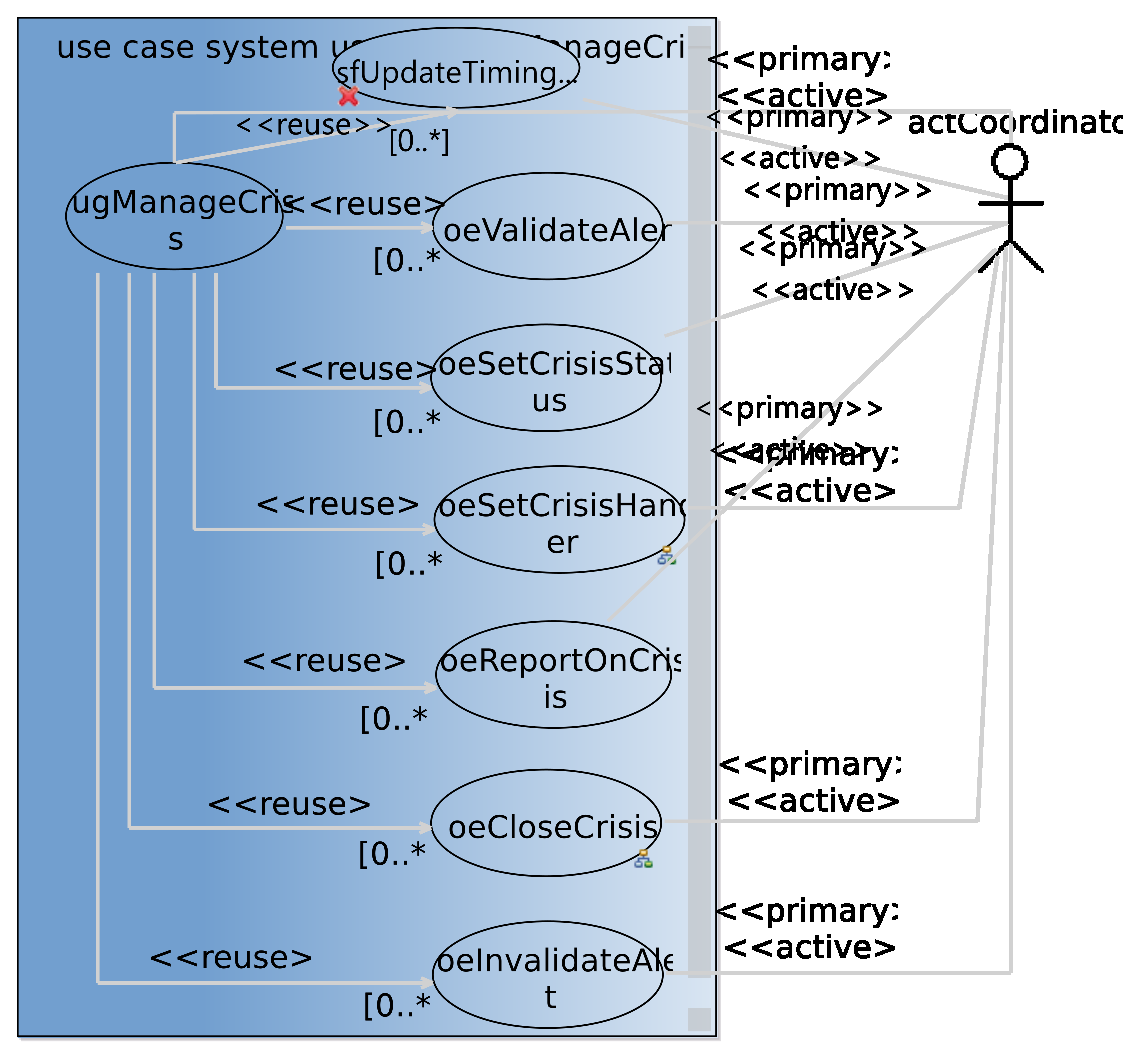
\includegraphics[
angle=0
,scale=0.75
]{./images-report-gen/usecase-model/usergoal/uc-ugManageCrisis.eps}
\end{center}
\caption[lu.uni.lassy.excalibur.examples.icrash Use Case Diagram: uc-ugManageCrisis]{ ugManageCrisis user goal use case}
\label{fig:lu.uni.lassy.excalibur.examples.icrash-RE-UCD-uc-ugManageCrisis}
\end{figure}
\vspace{0.5cm}
